\documentclass{article}

\usepackage{polski}
\usepackage[utf8]{inputenc}
\usepackage{graphicx}

 \usepackage{geometry} 
\newgeometry{tmargin=1.5cm, bmargin=1.5cm, lmargin=1.5cm, rmargin=1.5cm} 
\usepackage{enumerate}
\usepackage{setspace}
\usepackage{amsmath}
\usepackage{amssymb}
\usepackage{caption}
\usepackage{multirow}
\usepackage{mathtools}
\usepackage[utf8]{inputenc}
\usepackage{circuitikz}
\usepackage{cancel}
\usetikzlibrary{decorations.pathmorphing,arrows,snakes}
\usepackage{rotating}
\usepackage{gnuplottex}
\usepackage{pgf}
\usetikzlibrary{circuits.logic.US,circuits.logic.IEC}
\usepackage{latexsym}
\setlength\parindent{0pt}
\usepackage{ifthen}
\usepackage{keyval}
\usepackage{moreverb}
\usepackage{polski}
\usepackage{epstopdf}
\usepackage{pgfplots}
\newtheorem{definition}{Definicja}[section]
\usepackage{graphicx}
\renewcommand{\figurename}{Rys.}
\renewcommand{\tablename}{Tab.}

\graphicspath{{include/}}

\begin{document}

\begin{enumerate}
{\Large \bf  \item Scharakteryzuj obszary zastosowań badań nieniszczących w produkcji
przemysłowej.} [Damian H.]

{\Large \bf  \item Scharakteryzuj związki między fizycznymi i psychologicznymi parametrami fali
dźwiękowej.} [Damian H.]

{\Large \bf  \item Omów dwie znane Ci nieniszczące metody badania materiałów oparte o
wykorzystanie fal akustycznych.} [Jakub B.]

 

Wykorzystanie w tym celu fal ultradźwiękowych (wysoka częstotliwość drgań).
np.:

\begin{itemize}
\item Metoda cienia (transmisyjna):

Wymaga użycia dwóch przetworników i transmisji fali od jednego przetwornika do drugiego poprzez badany obszar materiału. Rejestrujemy wtedy natężenie fali przechodzącej przez materiał, a każda nieciągłość powoduje iż w rejestrowanym sygnale powstaje cień. (każda wada materiału powoduje odbicie lub osłabia fale). Nie daje nam jednak informacji gdzie dokładnie (na jakiej głębokości) znajduje się defekt. Nadaje się do badania przedmiotów o grubości maksymalnie 5 cm. 

\item Metoda echa (wykład)


\item Metoda emisji akustycznej 

W badanym elemencie "przykładamy"  zewnętrzną siłę w badanym elemencie (siła ta wytwarza w elemencie naprężenia oraz dyslokacje). Po usunięciu zewnętrznej siły element powraca do swojego stanu początkowego, a co za tym idzie wewnątrz powstają minimalne drgania o wysokiej częstotliwości (na powierzchni mogą powstawać wybrzuszenia). Na powierzchni powinny znajdować się czujniki które będą rejestrować dane zmiany i pozwolą zlokalizować  defekty lub tez nieciągłości materiału. Siłę  zewnętrzną możemy zastąpić nagłą zmiana temperatury lub też ciśnienia. 
( Rys prezentacja 2 slajd ostatni)

\begin{figure}[h!]
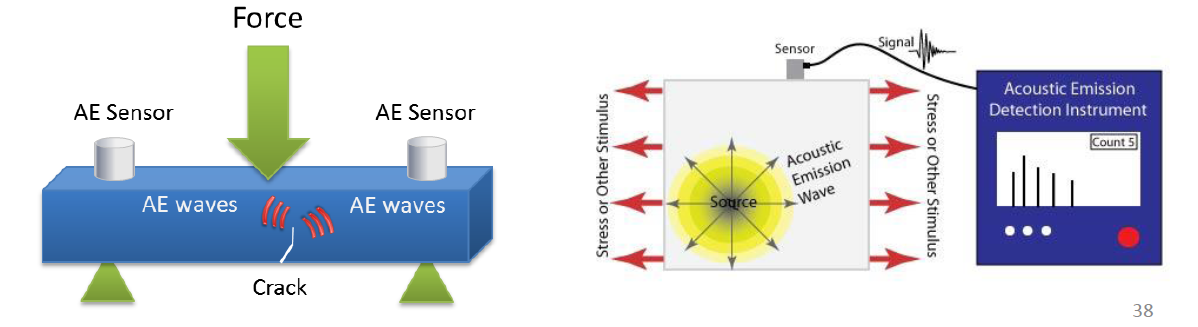
\includegraphics[width=\textwidth]{include/faleakust}
\end{figure}

\end{itemize}




{\Large \bf  \item Jakie znasz metody badań nieniszczących wykorzystujące pola magnetyczne?}  [Jakub B.]
 

W metodzie do badania nieciągłości na powierzchni elementów ferromagnetycznych,tej używa się proszków ferromagnetycznych  oraz pola magnetycznego pochodzącego od magnesu (lub tez elektromagnesu). 

Cząsteczki proszku ustawiają się wzdłuż linii pola magnetycznego, a więc największa ich ilość przypada w miejscu silnej zmiany pola magnetycznego. Pole magnetyczne przyłożone do materiału powoduje modyfikacje pola w obszarze nieciągłości w taki sposób iż tworzy się tam duży gradient pola. Jeżeli materiał jest wolny od wad linie te będą przebiegać bez zmian kierunku , jeśli natomiast w materiale jest wada w tym miejscu linie pola obrazowane przez proszek będą się odchylać. 
Jeżeli na powierzchni są zarysowania to proszek będzie się w nich oraz dookoła ich  silnie gromadzić. Proszki te zazwyczaj są pokolorowane lub tez mogą być fluorescencyjne co ułatwia badanie materiału. 

Metoda jest szybka łatwa oraz nie niszczy materiału ani go nie brudzi.
Wada: tylko dla materiałów ferromagnetycznych oraz konieczność wcześniejszego rozmagnesowania. 


{\bf Metoda wycieku strumienia magnetycznego }


Ponownie sposób badania materiału ferromagnetycznego. W urządzeniu znajduje się głowica z elektromagnesem która wytwarza pole magnetyczne oraz cewka która służy jako czujnik pola. Dodatkowym elementem jest przetwornik który monitoruje położenie głowicy. Całe urządzenie sprzężone jest z komputerem który analizuje prace urządzenia. Jeżeli w materiale znajduję się wada lub są odchyłki w grubościach są one rejestrowane przez sensor a komputer jest w stanie odtworzyć w którym miejscu znajdowała się wada. 








{\Large \bf  \item Scharakteryzuj nieniszczące metody badań oparte o zastosowanie promieniowania
jonizującego.} [Kamil W.]

{\Large \bf  \item Jakie znasz metody nieniszczących badań materiałowych oparte o zastosowanie
pól elektromagnetycznych?} [Zbigniew G.]

{\Large \bf  \item Podstawy fizyczne metody oznaczania składu elementarnego (spektroskopia
optyczna, XRF)} [Kamil S.]



Fluorescencja rentgenowska ( X - ray fluorescence = XRF) polega na wtórnej emisji promieniowania rentgenowskiego z materii, która została wzbudzona (np. przez zjawisko fotoelektryczne) za pomocą wysokoenergetycznego promieniowania. Metoda ta oparta jest na fakcie, iż każdy pierwiastek zawarty w analizowanej próbce, w skutek wzbudzenia rentgenowskiego emituje charakterystyczne dla siebie widmo.\\

{\bf Oddziaływanie promieniowania z materią}

Promieniowanie jest zdolne do oddziaływania z elektronami, jak i jądrami oraz z ich polami elektrycznymi. Na skutek tego oddziaływania może dojść do elastycznego i nieelastycznego rozpraszania promieniowania lub do całkowitej jego absorpcji. Jednakże najbardziej prawdopodobnymi i znaczącymi są następujące trzy zjawiska (punktu widzenia naszego doświadczenia najistotniejszym jest efekt fotoelektryczny):\\

{\bf Zjawisko fotoelektryczne}
Kwant promieniowania elektromagnetycznego (np. promieniowania $\gamma$ lub promieniowania X) padając na atom przekazuje całą swoją energie $\hbar\omega$ elektronowi z powłoki wewnętrznej. Elektron ten dzięki pozyskanej energii może opuścić atom pokonując energię wiązania $E_B$ na orbicie. Jeżeli energia padającego kwantu jest większa niż $E_B$ to pozostała jej część staje się energią kinetyczną $T_e$ wybitego elektronu:
\begin{gather*}
\hbar\omega=T_e+E_B
\end{gather*}
W miejsce wybitego elektronu spada elektron z wyższej orbity emitując jednocześnie kwant promieniowania o energii równej różnicy poziomów energetycznych obu orbit.
\begin{gather*}
\hbar\omega'=E_i-E_f
\end{gather*}

\begin{center}
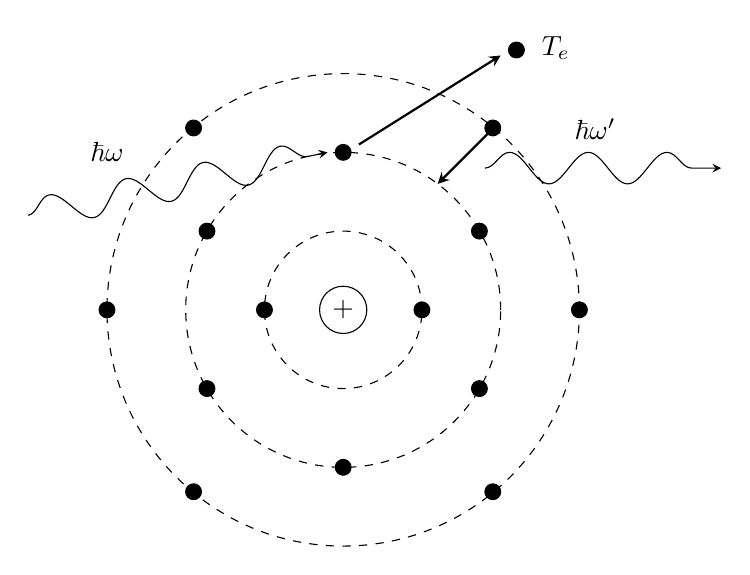
\begin{tikzpicture}
\draw[-stealth,
decoration={snake,
    amplitude = 2mm,
    segment length = 10mm,
    post length=0.4mm},decorate] (-4,1.2) -- (-0.2,2);
\draw [-stealth, thick] (0.2,2.1) -- (2,3.23);
\draw [-stealth, thick] (1.9,2.3) -- (1.2,1.6);
\draw[-stealth,
decoration={snake,
    amplitude = 2mm,
    segment length = 10mm,
    post length=0.4mm},decorate] (1.8,1.8) -- (4.8,1.8);
\draw (0,0) circle [radius=0.3] node {+};
\filldraw[fill=black, draw=black] (2.2,3.3) circle [radius=0.1];
\draw[dashed] (0,0) circle [radius=1];
\draw[dashed] (0,0) circle [radius=2];
\draw[dashed] (0,0) circle [radius=3];
\filldraw[fill=black, draw=black] (1,0) circle [radius=0.1];
\filldraw[fill=black, draw=black] (-1,0) circle [radius=0.1];
\filldraw[fill=black, draw=black] (0,2) circle [radius=0.1];
\filldraw[fill=black, draw=black] (0,-2) circle [radius=0.1];
\filldraw[fill=black, draw=black] (1.73,1) circle [radius=0.1];
\filldraw[fill=black, draw=black] (-1.73,1) circle [radius=0.1];
\filldraw[fill=black, draw=black] (1.73,-1) circle [radius=0.1];
\filldraw[fill=black, draw=black] (-1.73,-1) circle [radius=0.1];
\filldraw[fill=black, draw=black] (3,0) circle [radius=0.1];
\filldraw[fill=black, draw=black] (-3,0) circle [radius=0.1];
\filldraw[fill=black, draw=black] (1.9,2.31) circle [radius=0.1];
\filldraw[fill=black, draw=black] (-1.9,2.31) circle [radius=0.1];
\filldraw[fill=black, draw=black] (-1.9,-2.31) circle [radius=0.1];
\filldraw[fill=black, draw=black] (1.9,-2.31) circle [radius=0.1];
\node (A) at (-3,2) {$\hbar\omega$};
\node (B) at (3.2,2.3) {$\hbar\omega'$};
\node (C) at (2.7,3.32) {$T_e$};
\end{tikzpicture}
\end{center}

Linie emisyjne powstałe w skutek tego zjawiska są charakterystyczną cechą pierwiastków, więc doskonale nadają się do ich identyfikacji. Serie linii emisyjnych oznaczane są z powszechnie stosowaną symboliką odpowiednio: K, dla przejść na powłokę o głównej liczbie kwantowej n=1, L dla n=2, M dla n=3 itd. Linie widmowe dla poszczególnych przejść oznacza się symbolem serii i literą grecką $\alpha$ dla przejść o $\Delta n =1$, $\beta$ dla $\Delta n=2$ itd. wraz z kolejnymi cyframi arabskimi.
Jest to jeden ze sposobów uzyskania fluorescencji.\\
{\bf Rozpraszanie Comptona}

Rozpraszanie Comptona polega na nieelastycznym rozpraszaniu kwantów $\gamma$ na swobodnych elektronach (zakładamy, że elektrony z powłok zewnętrzych są swobodne, ponieważ $E_{\gamma}\gg E_B$). Na skutek tego zjawiska foton zmienia swój kierunek ruchu jak i energię (tym samym długość fali). Foton traktujemy tutaj jako cząstek o energii i pędzie zdefiniowanych jako:
 \begin{gather*}
E_{\gamma}=\hbar\omega, \quad \quad \quad p_{\gamma}=\frac{\hbar\omega}{c}
\end{gather*}
\begin{minipage}[h]{0.5\linewidth}
\centering
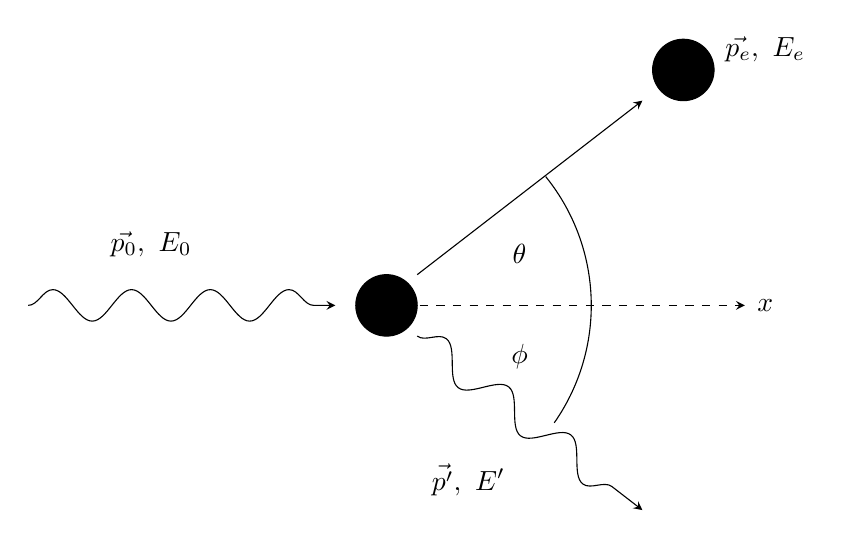
\begin{tikzpicture}[scale=1.3]

\coordinate (0) at (0,0);
\coordinate (A) at (2.5,0);
\coordinate (B) at (2,-1);

\draw[-stealth,
decoration={snake,
    amplitude = 2mm,
    segment length = 10mm,
    post length=0.4mm},decorate] (-3,0) -- (0,0);
\filldraw [fill=black,draw=black] (0.5,0) circle [radius=0.3];
\filldraw [fill=black,draw=black] (3.4,2.3) circle [radius=0.3];
\draw [-stealth,dashed] (0.5,0) -- (4,0);
\draw [-stealth] (0.8,0.3) -- (3,2);
\draw[-stealth,
decoration={snake,
    amplitude = 2mm,
    segment length = 10mm,
    post length=0.4mm},decorate] (0.8,-0.3) -- (3,-2);
\draw [black](A) arc (0:39:2);
\draw [black](A) arc (0:-35:2);

\node (A) at (1.8,0.5) {$\theta$};
\node (B) at (1.8,-0.5) {$\phi$};
\node (C) at (4.2,2.5) {$\vec{p_e},\ E_e$};
\node (D) at (-1.8,0.6) {$\vec{p_0},\ E_0$};
\node (E) at (1.3,-1.7) {$\vec{p'},\ E'$};
\node (F) at (4.2,0) {$x$};
\end{tikzpicture}
\end{minipage}
\begin{minipage}[h]{0.5\linewidth}
\centering
W procesie tym muszą być spełnione zasada zachowania energii oraz pędu:\\ 
 \begin{gather*}
E_0+m_oc^2=E_e+E'\\
p'\cos{\phi}+p_e\cos{\theta}=p_0\\
p_e\sin{\theta}=p'\sin{\phi}
\end{gather*}
\end{minipage}

\vspace{0.5cm}
Uzyskujemy zmianę długości fali kwantu $\gamma$ daną wzorem:
 \begin{gather*}
\Delta\lambda=\lambda'-\lambda_0=\frac{h}{m_0c}(1- cos{\phi})
\end{gather*}

zmiana energii dana jest zależnością:
 \begin{gather*}
\frac{1}{E'}=\frac{1}{E_{0}}+\frac{1}{m_0c^2}(1- cos{\phi})
\end{gather*}



{\bf Kreacja pary cząstka - antycząstka}

Kwant promieniowania $\gamma$ może wykreować parę cząstek w postaci elektronu $e^-$ i pozytonu $e^+$, w polu kulombowskim elektronu lub jądra, jeżeli spełni warunek energetyczny:
 \begin{gather*}
\hbar\omega >2m_0c^2 = 1.022\ MeV
\end{gather*}
Obecność dodatkowej cząstki jest konieczna ze względu na fakt, iż w układzie foton - para elektronów nie mogą być równocześnie  spełnione prawa zachowania energii i pędu. Stosując oba prawa możemy uzyskać wzór na energię kwantu $\gamma$ potrzebną do wytworzenia pary w pobliżu cząstki o masie M:
 \begin{gather*}
E_{\gamma}=2m_ec^2\left ( 1+\frac{m_e}{M} \right )
\end{gather*}
\begin{center}
\begin{tikzpicture}[scale=1]

\coordinate (0) at (0,0);
\coordinate (A) at (2.5,0);
\coordinate (B) at (2,-1);

\draw[-stealth,
decoration={snake,
    amplitude = 2mm,
    segment length = 10mm,
    post length=0.4mm},decorate] (-3,0) -- (0,0);
\draw (0.35,0.3) circle [radius=0.3] node {+};
\filldraw [fill=black,draw=black] (2,1.2) circle [radius=0.1];
\filldraw [fill=black,draw=black] (2,-1.2) circle [radius=0.1];

\draw [-stealth] (0.8,0.2) -- (3,2);
\draw[-stealth] (0.8,-0.2) -- (3,-2);


\node (D) at (-1.8,0.6) {$\hbar\omega$};
\node (E) at (2.4,-1.1) {$e^+$};
\node (C) at (2.4,1.1) {$e^-$};
\node (B) at (0.35,0.8) {$M$};
\end{tikzpicture}
\end{center}



{\bf Spektroskopia optyczna}

Do analizy składu możemy wykorzystać nie tylko promieniowanie w zakresie rentgenowskim, ale również światło z zakresu widzialnego. W celu otrzymania widma pierwiastka należy przez próbkę przepuścić światło białe lub spowodować jej wzbudzenie (łukiem elektrycznym, przykładając wysokie napięcie, spalając sole danego pierwiastka w palniku). Do wyjaśnienia powstawania widm możemy posłużyć się modelem atomu Bohra, na podstawie którego wiemy  że przejściu elektronu między orbitami towarzyszy wypromieniowanie energii równej różnicy energii tych dwóch orbitali:
\begin{gather*}
\hbar\omega=E_i-E_f
\end{gather*}
W zależności od sposobu powstania oraz wyglądu wyróżniamy następujące widma:
\begin{itemize}
\item Widma absorpcyjne - powstaje podczas przechodzenia promieniowania przez ośrodek, który to absorbuje jedynie  fale o ściśle określonej energii, co związane jest z charakterystycznym ułożeniem poziomów energetycznych, na które mogą  przechodzić elektrony tego ośrodka.

\begin{figure}[h!]
\centering
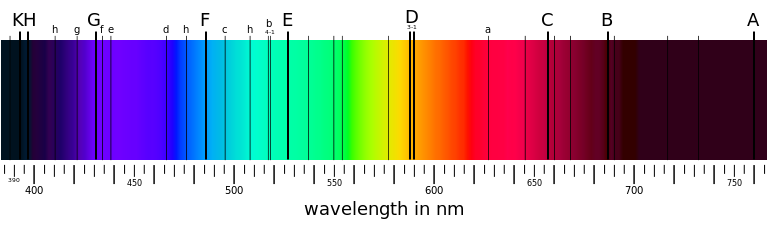
\includegraphics[scale=0.5]{absorpcja.png}
\caption{Widmo absorpcyjne}
\end{figure}

\item Widma emisyjne - powstaje na skutek wysyłania przez próbkę promieniowania. Badaną próbkę  na początku wzbudza się np. łukiem elektrycznym, spalając w palniku itp. dzięki czemu elektrony przechodzą do wyższego stanu energetycznego, a następnie wracając do stanu podstawowego emitują ściśle określoną energię równą różnicy energii tych dwóch poziomów.

\begin{figure}[h!]
\centering
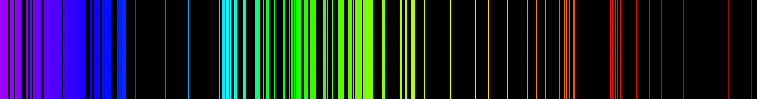
\includegraphics[scale=0.5]{emisja.png}
\caption{Widmo emisyjne żelaza}
\end{figure}

\item Widma ciągłe - ma postać ciągłego obszaru lub szerokich pasów. Charakterystyczne dla ciał stałych i cieczy.
\item Widma liniowe - ma postać oddzielnych linii na pasku widmowym. Jest ono typowe dla gazów atomowych.
\item Widma pasmowe - przypadek pośredni pomiędzy liniowym a ciągłym. Można je zaobserwować dla gazowych związków chemicznych. Pasma powstają tam na skutek zlewania się poszczególnych linii pochodzących od sąsiadujących ze sobą licznych poziomów energetycznych rotacyjno - oscylacyjnych. 
\end{itemize}

{\Large \bf  \item Mikroskopia elektronowa (transmisyjna i skaningowa)} [Kamil S.]
{\bf Mikroskopia elektronowa}\\

Zdolność rozdzielczą mikroskopu można przedstawić wzorem:
\begin{gather*}
R=0.61\cdot \frac{\lambda}{A}
\end{gather*}
\begin{flushright}
\small
$\lambda$ - długość fali promieniowania\\
$ A$ - apertura mikroskopu
\end{flushright}
Chcąc uzyskiwać coraz to większe rozdzielczości koniecznym było znalezienie źródła fal o krótszych długościach. W 1924 de Brogile zapostulował dwoistą naturę korpuskularno - falową elektronów podając swój słynny wzór wiążący długość fali z pędem cząstki:
\begin{gather*}
\lambda=\frac{\hbar}{p}
\end{gather*}
Podstawowym elementem mikroskopu elektronowego jest kolumna zawierająca źródło elektronów (np. wolfram, działo z emisją polową). Wstępnie ukształtowana wiązka elektronów zostaje rozpędzona w obszarze między katodą a anodą uzyskując energię:
\begin{gather*}
E=eU
\end{gather*}
Obecność wysokiej próżni w kolumnie pozwala na swobodne poruszanie się elektronów od działa do ekranu. Wiązka po drodze do próbki przechodzi przez szereg soczewek magnetycznych i kolimatorów, które ją kształtują oraz pozwalają na płynną zmianę jej biegu. Następnie wiązka elektronów pada na próbkę oddziałując z jego materią. Elektrony, które przeszły przez próbkę są skupiane przez układ soczewek i trafiają  na detektor. \\

{\bf Oddziaływanie elektronów z próbką}\\

Elektrony padające na próbkę zderzają się z jej atomami, w wyniku czego tracą energię kinetyczną, ulegają pochłonięciu, odbiciu lub powodują emisję promieniowania. Większość energii zamieniana jest jednak na ciepło (wraz ze wzrostem liczby atomowej maleje liczba elektronów pochłoniętych, a rośnie odbitych). W wyniku oddziaływania elektronów pierwotnych z próbką emitowane są różne rodzaje elektronów oraz promieniowania, które wykorzystuje się w analizie składu oraz do tworzenia obrazu:
\begin{itemize}
\item {\bf Elektrony wtórne (SE - Secondary Electrons)} - w dużym stopniu są to elektrony, pochodzące z atomów występujących blisko powierzchni ciała stałego, wyemitowane w wyniku zderzeń z~elektronami wiązki pierwotnej. Elektronami wtórnymi mogą być także elektrony pierwotne, które straciły całą energię przy rozpraszaniu i wydostały się z powierzchni. Ich gęstość  (liczba wyemitowanych przez elektron pierwotny), zależy od napięcia przyspieszającego.
\item {\bf Elektrony wstecznie rozproszone (BSE - Backscattered Electrons)} - to elektrony pierwotne ulegające odbiciu sprężystemu od jąder atomowych próbki i opuszczające powierzchnię oddziaływania z niewielką zmianą energii kinetycznej. Wydajność tych elektronów $\eta$ nie zależy od napięcia przyspieszającego i jest niewielka w stosunku do gęstości. Podobnie jak poprzednicy (elektrony wtórne) wykorzystuje się je również do tworzenia obrazu w SEM, gdyż $\eta$ jest silnie powiązane z liczbą atomową Z . Dlatego też w celu rozróżnienia faz różniących się liczbą atomową, stosuje się technikę obrazowania z elektronami wstecznie rozproszonymi BSE.

\item {\bf Elektrony Augera i promieniowanie rentgenowskie} - elektrony Augera generowane są z niewielkiej głębokości próbki . Wiązka pierwotna powoduje wzbudzenie atomu przez wybicie elektronu z powłoki wewnętrznej, po czym powraca on do stanu równowagi na skutek przeskoku elektronu z poziomu o wyższej energii na wolne miejsce na powłoce wewnętrznej . Podczas tego zjawiska uwalniany jest nadmiar energii ($\Delta E$) związany z różnicą energii między poziomami energetycznymi elektronów. Wyemitowana różnica energii może przyczynić się do emisji nisko energetycznych (100-1000 eV) elektronów Augera (z poziomów zewnętrznych), promieniowania rentgenowskiego  bądź fotonów światła widzialnego o długości fali $\lambda = hc/\Delta E$ . Elektrony Augera są bardzo ważne w analizie składu chemicznego warstw powierzchniowych . Charakterystyczne dla danego pierwiastka energia i długość fali promieniowania rentgenowskiego, są również wykorzystywane do analizy składu chemicznego .
\end{itemize}

W zależności od tego, które z oddziaływań chcemy wykorzystać do obrazowania i detekcji możemy wyróżnić dwa podstawowe rodzaje mikroskopów elektronowych:
\begin{itemize}
\item {\bf Transmisyjny mikroskop elektronowy (TEM)} - przyrząd stosowany w celu prześwietlania próbki za pomocą wytworzonej w nim i odpowiednio uformowanej wiązki elektronów.  Wewnątrz kolumny znajduje się źródło elektronów , szereg urządzeń formujących wiązkę, ekran, miejsce do umieszczania próbek , czy urządzenie rejestrujące obrazy. Dodatkowo wszystko dopełniają układy wysokiego napięcia oraz próżniowy. W związku z faktem, iż interesują nas głównie elektrony, które przeszły przez badany materiał to próbki wykorzystywane w TEM powinny być cienkimi warstwami. W takich cienkich warstwach energia elektronów przechodzących jest wytracana podczas oddziaływań z elektronami próbki (rozpraszanie nieelastyczne) bądź nie zmieniając swojej energii elektrony pierwotne zmieniają kierunek lotu w wyniku oddziaływania z jądrami (oddziaływanie elastyczne). W przypadku rozpraszania nieelastycznego, jego intensywność uzależniona jest od składu chemicznego, gęstości i grubości próbki. 

\begin{figure}[h!]
\centering
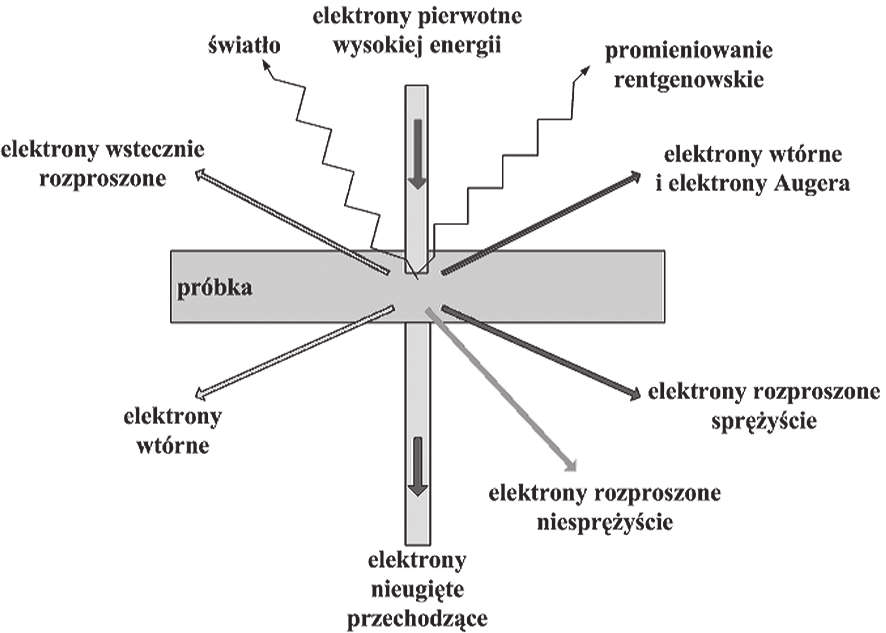
\includegraphics[scale=0.3]{oddzialywanie.png}
\caption{Schemat przedstawiający oddziaływanie elektronu z materią w przypadku cienkiej próbki}
\end{figure}

\newpage
\begin{figure}[h!]
\centering
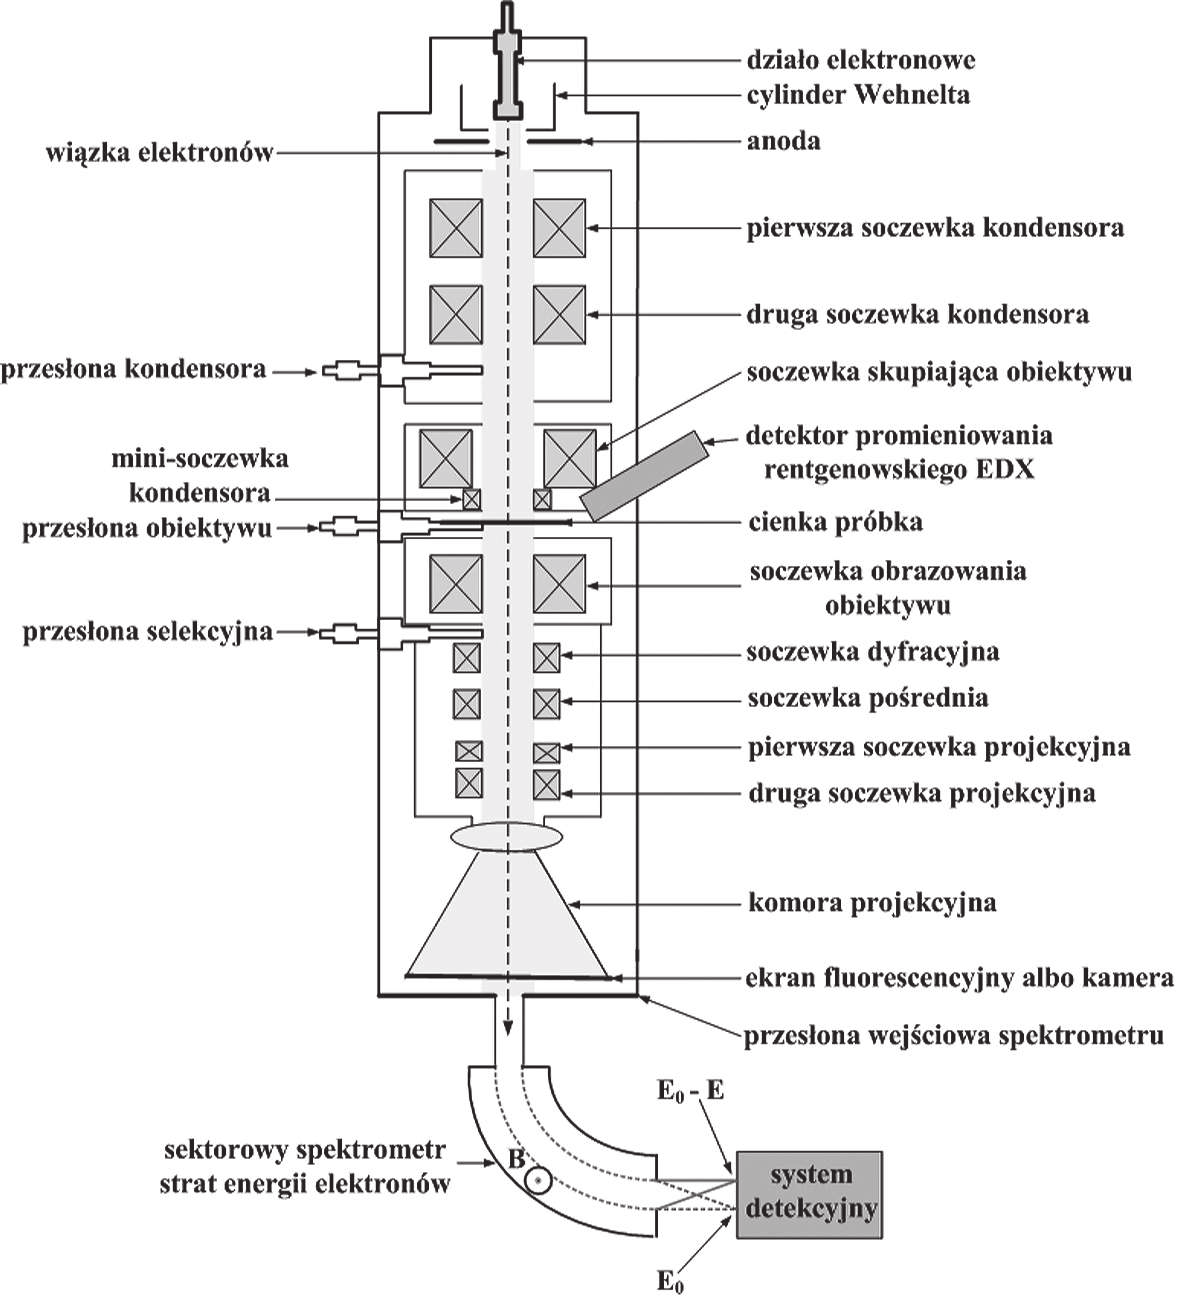
\includegraphics[scale=0.25]{tem.png}
\caption{Schemat budowy transmisyjnego mikroskopu elektronowego}
\end{figure}


\item {\bf Skaningowy mikroskop elektronowy (SEM)} - przyrząd pozwalający na obrazowanie powierzchni badanych próbek. Jego idea polega na skanowaniu powierzchni próbki nanometrową wiązką elektronów uformowaną przez elektrono - optyczny układ mikroskopu. Sygnał z powierzchnii próbki, zazwyczaj w postaci elektronów wtórnych albo odbitych, dociera do detektora, którego najważniejszymi częściami są scyntylator i fotopowielacz. Część elektronów z wiązki pierwotnej ulegają rozproszeniu wstecznemu (sprężyste rozpraszanie) blisko powierzchni próbki, emitując sygnał tzw. elektronów odbitych (BSE). Reszta rozprasza się niesprężyście przez powierzchniowe warstwy atomów, podczas czego emitowany jest najważniejszy w skaningowej metodzie sygnał pochodzący od nisko - energetycznych elektronów wtórnych. Elektrony te są szczególnie czułe na topografię powierzchni próbki. Stosowane w SEM próbki nie muszą być tak cienkie jak w przypadku TEM, a przez to ich przygotowanie nie jest skomplikowane.

\begin{figure}[h!]
\centering
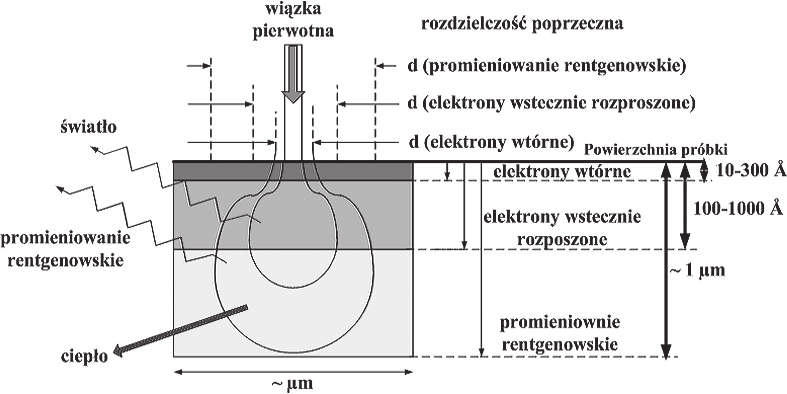
\includegraphics[scale=0.4]{gruszka.png}
\caption{Schemat oddziaływania elektronów z materią w grubej próbce}
\end{figure}


\begin{figure}[h!]
\centering
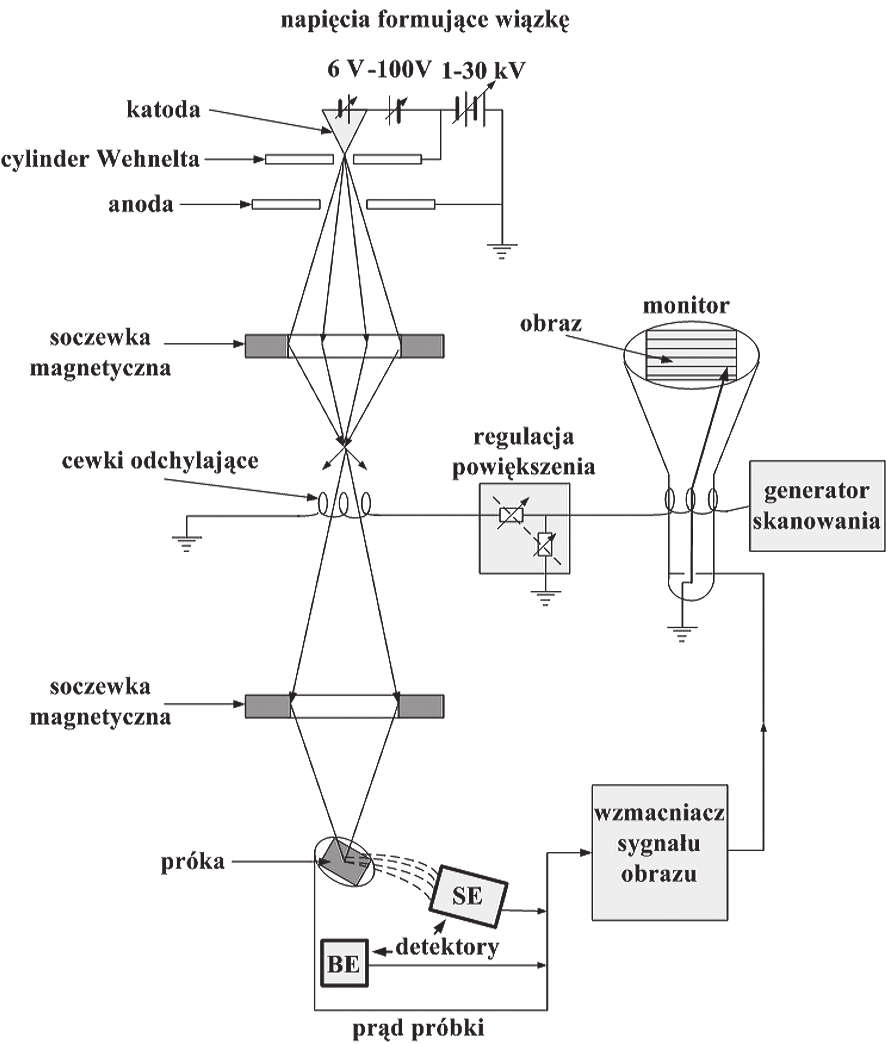
\includegraphics[scale=0.3]{sem.png}
\caption{Schemat budowy skaningowego mikroskopu elektronowego}
\end{figure}

\end{itemize}



















{\Large \bf  \item Definicje podstawowych jednostek układu SI} [Andrzej W.]

Układ SI definiuje siedem jednostek miary jako podstawowy zbiór z których tworzone są jednostki pochodne. Te podstawowe jednostki i ich fizyczna wielkość to:
\begin{itemize}
\item    metr – długość
\item     kilogram – masa (uwaga: nie gram)
\item     sekunda – czas
\item     amper – prąd elektryczny
\item     kelwin – temperatura
\item     kandela – światłość
\item     mol – liczność materii
\end{itemize}

{\bf Definicje podstawowych jednostek:}

{\small
\begin{tabular}{cccll}
\hline
\hline
nazwa & symbol & wielkość & def. współczesna & def. historyczna \\ 
\hline
\hline
 &&&odległość, jaką pokonuje światło &$\displaystyle\frac{1}{10^7}$ długości mierzonej wzdłuż\\
metr & m & długość &w próżni w czasie 1/299 792 458 s. &  południka paryskiego \\
&&&&od równika do bieguna.\\
\hline
kilogram&	kg&	masa&	masa międzynarodowego wzorca kilograma
&	Masa jednego litra wody.\\
\hline
&&&	czas równy 9 192 631 770 okresom &\\
&&&promieniowania odpowiadającego przejściu \\ 
sekunda&	s&	czas&między dwoma poziomami F = 3 i F = 4&sekunda to 1/(24$\cdot$60$\cdot$60) doby\\
&&& struktury nadsubtelnej stanu podstawowego\\
&&& $^2S_{1/2}$ atomu cezu $^{133}$Cs”\\
 &&&(w spoczynku w temperaturze 0 K)\\
 \hline
	&&& natężenie  prądu elektrycznego,& zdef. elektrochemicznie jako  \\
&&&który płynąc w dwóch równoległych, & prąd potrzebny do wytrącenia\\
&&&prostoliniowych, nieskończenie długich  &  1.118 [mg] srebra na [s] z roztworu\\
amper&	A&	prąd elek.&przewodach,  umieszczonych w próżni& azotanu srebra. W porównaniu\\
&&& w odległości 1 m od siebie, spowodowałby& do obecnej definicji, różnica \\
&&& wzajemne oddziaływanie przewodów&wynosi 0,015\%.\\
&&& na siebie z siłą równą $2\cdot10^{-7}$ N \\
\hline
&&&jeden kelwin to jednostka temperatury&Skala Celsjusza: skala Kelvina \\
&&& równa 1/273,16 temperatury&opiera się na skali Celsjusza,\\
kelwin&	K	&temperatura& termodynamicznej punktu potrójnego wody.”&lecz jest skalą termodynamiczną\\
&&& (woda: 0,00015576 mola $^2$H na jeden mol $^1$H,& (0 K to zero bezwzględne).\\
&&& 0,0003799 mola $^{17}$O na jeden mol $^{16}$O\\
&&& i 0,0020052 mola ${^18}$O na jeden mol $^{16}$O\\
\hline
&&&	liczność materii układu, zawierającego\\
&&& liczbę cząstek równą liczbie atomów& Masa cząsteczkowa \\
&&& zawartych w dokładnie 0,012 kg izotopu&podzielona przez 1 g/mol.\\
mol&	mol&	liczność materii& węgla $^{12}$C. W definicji zakłada się, że \\
&&&węgiel jest w stanie niezwiązanym chemicznie,\\
&&& w spoczynku, a jego atomy nie znajdują\\
&&& się w stanie wzbudzenia.”\\
\hline

&&&	 światłość z jaką świeci w określonym\\
&&& kierunku źródło emitujące promieniowanie\\
kandela&	cd&	światłość& monochromatyczne o częstotliwości&Wcześniejszą jednostką\\
&&& 5,4·1014 Hz i wydajności energetycznej&światłości była świeca.\\
&&& w tym kierunku równej\\
&&& (1/683) [W] na [srad]\\
\hline\hline	
  
\end{tabular}
}


{\Large \bf  \item Podstawowe fakty historyczne związane ze współpracą międzynarodową w
zakresie ustalenia jednolitych jednostek miar.} [Andrzej W.]


{\bf I Generalna Konferencja Miar} z 26 września 1889 r. ustaliła (obowiązującą do 1960 r.) {\bf definicję metra} jako odległości w temperaturze 0$^\circ$C i przy normalnym ciśnieniu atmosferycznym między dwiema głównymi {\bf kreskami na platynowoirydowym wzorcu}, złożonym w Międzynarodowym Biurze Miar w Sèvres pod Paryżem, oraz (nadal obowiązującą) {\bf definicję i wzorzec kilograma}.

{\bf IX Generalna Konferencja Miar} w 1948 r. rozpisała ankietę dotyczącą wprowadzenia nowego układu miar po szeregu krytycznych studiów na temat dotychczasowego (niedoprecyzowanego) układu (w szczególności miano wybrać czwartą jednostkę podstawową, dla pomiaru wielkości elektrycznych, spośród sześciu zaproponowanych). Wprowadziła {\bf (nadal obowiązującą) definicję ampera}, jako jednej z proponowanych w ankiecie jednostek. Ustaliła (obowiązującą do 1979 r., z drobną poprawką) definicję kandeli.

{\bf X Generalna Konferencja Miar} w 1954 r. ustanowiła sześć jednostek podstawowych (metr, kilogram, sekunda, amper, kandela, stopień Kelvina), i przyjęła zasadę spójności układu jednostek podstawowych. Wybrała amper, jako elektryczną jednostkę podstawową. Ustaliła (nadal obowiązującą, z późniejszą poprawką) definicję stopnia Kelvina (nazwa zmieniona w 1967 r.). Wprowadziła definicję jednostki ciśnienia – atmosfery fizycznej.

{\bf XI Generalna Konferencja Miar} w Paryżu w październiku 1960 r. ustanowiła ostatecznie międzynarodowy układ jednostek, wprowadzając dlań {\bf skrót SI} (Système International d'Unités). Zatwierdziła (obowiązującą do 1967 r.) definicję sekundy, używaną obecnie tylko dla celów astronomicznych jako 1/31 556 925,9747 część roku zwrotnikowego 1900 stycznia 0 godzina 12:00, czasu efemeryd. Przyjęła nową (obowiązującą do 1983 r.) definicję metra jako długości równej 1 659 763,73 długości fali promieniowania w próżni odpowiadającego przejściu między poziomami $2$p$^{10}$ a 5d$^5$ atomu $^{86}$Kr. {\bf Oficjalnie wprowadzono przedrostki.}


XIII Generalna Konferencja Miar w październiku 1967 r. wprowadziła nową nazwę jednostki temperatury – kelwin i drobną poprawkę w jej definicji. Przyjęła nową (obecnie obowiązującą) definicję sekundy, opartą na wzorcu odtwarzalnym w warunkach laboratoryjnych. Wprowadziła przeliczenie jednostki ciśnienia atmosfery fizycznej na jednostki SI. Wprowadziła drobną poprawkę w definicji kandeli, uwzględniającą to przeliczenie.

{\bf XIV Generalna Konferencja Miar} w październiku 1971 r. wprowadziła do układu SI, jako jego siódmą jednostkę podstawową, jednostkę ilości (liczności) substancji {\bf mol}, i przyjęła jej (obecnie obowiązującą) definicję. Zatwierdziła nową nazwę jednostki ciśnienia – paskal.

{\bf XVI Generalna Konferencja Miar} w październiku 1979 r. przyjęła {\bf nową (obecnie obowiązującą) definicję kandeli}.

{\bf XVII Generalna Konferencja Miar} w październiku 1983 r. przyjęła (21 X) {\bf nową (obecnie obowiązującą) definicję metra}.

 
 




{\Large \bf  \item Z jakimi metodami fizycznymi zapoznałeś się przy badaniu materiałów węglowo-
grafitowych (SGL-Racibórz)} [Kamil W.]
\end{enumerate}



\end{document}